%%
%% Beginning of file 'sample.tex'
%%
%% Modified 2005 December 5
%%
%% This is a sample manuscript marked up using the
%% AASTeX v5.x LaTeX 2e macros.

%% The first piece of markup in an AASTeX v5.x document
%% is the \documentclass command. LaTeX will ignore
%% any data that comes before this command.

%% The command below calls the preprint style
%% which will produce a one-column, single-spaced document.
%% Examples of commands for other substyles follow. Use
%% whichever is most appropriate for your purposes.
%%
%%\documentclass[12pt,preprint]{aastex}

%% manuscript produces a one-column, double-spaced document:

\documentclass[manuscript]{aastex}

%% preprint2 produces a double-column, single-spaced document:

%% \documentclass[preprint2]{aastex}

%% Sometimes a paper's abstract is too long to fit on the
%% title page in preprint2 mode. When that is the case,
%% use the longabstract style option.

%% \documentclass[preprint2,longabstract]{aastex}

%% If you want to create your own macros, you can do so
%% using \newcommand. Your macros should appear before
%% the \begin{document} command.
%%
%% If you are submitting to a journal that translates manuscripts
%% into SGML, you need to follow certain guidelines when preparing
%% your macros. See the AASTeX v5.x Author Guide
%% for information.

\newcommand{\vdag}{(v)^\dagger}
\newcommand{\myemail}{skywalker@galaxy.far.far.away}

%% You can insert a short comment on the title page using the command below.
\usepackage[a4paper=true,dvipdfm=true]{hyperref}
\usepackage{multirow}
\slugcomment{Not to appear in Nonlearned J., 45.}

%% If you wish, you may supply running head information, although
%% this information may be modified by the editorial offices.
%% The left head contains a list of authors,
%% usually a maximum of three (otherwise use et al.).  The right
%% head is a modified title of up to roughly 44 characters.
%% Running heads will not print in the manuscript style.

\shorttitle{On the Construction of New Stellar  Classification Template Library for LAMOST Spectra Analysis Pipeline}
\shortauthors{Peng Wei, Ali Luo et al.}

%% This is the end of the preamble.  Indicate the beginning of the
%% paper itself with \begin{document}.

\begin{document}

%% LaTeX will automatically break titles if they run longer than
%% one line. However, you may use \\ to force a line break if
%% you desire.

\title{On the Construction of New Stellar  Classification Templates Library for LAMOST Spectra Analysis Pipeline}

%% Use \author, \affil, and the \and command to format
%% author and affiliation information.
%% Note that \email has replaced the old \authoremail command
%% from AASTeX v4.0. You can use \email to mark an email address
%% anywhere in the paper, not just in the front matter.
%% As in the title, use \\ to force line breaks.


%% Notice that each of these authors has alternate affiliations, which
%% are identified by the \altaffilmark after each name.  Specify alternate
%% affiliation information with \altaffiltext, with one command per each
%% affiliation.

\author{Peng Wei\altaffilmark{1, 2}, Ali Luo*\altaffilmark{1, 3}, Yinbi Li\altaffilmark{1}, }
\affil{Key Laboratory of Optical Astronomy, National Astronomical Observatories,   Chinese Academy of Sciences,  Beijing,  100012,  China}
\email{lal@nao.cas.cn weipeng@nao.cas.cn}

\author{Jingchang Pan\altaffilmark{3},Bin Jiang \altaffilmark{3}, }
\affil{School of Mechanical,  Electrical and Information Engineering,  Shandong University, Weihai,  264209,  China}

\author{Fengfei Wang\altaffilmark{1}, Jiannan Zhang\altaffilmark{1}, Liangping Tu \altaffilmark{1, 4}, Yongheng Zhao\altaffilmark{1}, Jianjun Chen\altaffilmark{1, 2}, Xiaoyan Chen\altaffilmark{1}, Bing Du\altaffilmark{1}, Yanxin Guo\altaffilmark{1}, Wen Hou\altaffilmark{1, 2}, , Xiao Kong\altaffilmark{1, 2}, Juanjuan Ren \altaffilmark{1, 2}, Yihan Song\altaffilmark{1}, Mengxin Wang\altaffilmark{1}, Yue Wu\altaffilmark{1}, Haifeng Yang \altaffilmark{1, 2, 5}, Fang Zuo\altaffilmark{1}, }
\affil{Key Laboratory of Optical Astronomy, National Astronomical Observatories,   Chinese Academy of Sciences,  Beijing,  100012,  China}

\author{Jie Liu\altaffilmark{3}, Zhenping Yi\altaffilmark{1, 2, 3}, }
\affil{School of Mechanical,  Electrical and Information Engineering,  Shandong University, Weihai,  264209,  China}

\author{Ge Jin\altaffilmark{6}}
\affil{University of Science and Technology of China,  Hefei 230026,  China}
\altaffiltext{1}{Key Laboratory of Optical Astronomy,National Astronomical Observatories,  Chinese Academy of Sciences, Beijing, 100012, China}
\altaffiltext{2}{University of Chinese Academy of Sciences, Beijing, 100049, China}
\altaffiltext{3}{School of Mechanical, Electrical and Information Engineering, Shandong University,Weihai, 264209, China}
\altaffiltext{4}{School of Science, Liaoning University of Science and Technology,  Anshan, 144051, China}
\altaffiltext{5}{School of Computer Science and Technology, Taiyuan University of Science and Technology,Taiyuan 030024, China}
\altaffiltext{6}{University of Science and Technology of China, Hefei 230026, China}

%% Mark off your abstract in the ``abstract'' environment. In the manuscript
%% style, abstract will output a Received/Accepted line after the
%% title and affiliation information. No date will appear since the author
%% does not have this information. The dates will be filled in by the
%% editorial office after submission.

\begin{abstract}
The LAMOST spectra analysis pipeline is one of LAMOST softwares to produce and analyze spectra,
and its aim is to classify and measure the spectra observed in the survey.
Through this pipeline, the observed stellar spectra are classified into different sub-classes by matching with templates spectra.
Consequently, the performance of the stellar classification greatly depends on the quality of template spectra.
%This paper presents the construction of the new stellar classification templates library for the LAMOST Spectra Analysis Pipeline.
%A new LAMOST stellar spectral classification template library is constructed, which is supposed to  improve the precision  and credibility  of the stellar classification.
In this paper,
we construct a new LAMOST stellar spectral classification template library,
which is supposed to  improve the precision  and credibility  of the present LAMOST stellar classification.
About one million spectra are selected from LAMOST Data Release one (DR1) to construct the new stellar templates,
and they are gathered in 233 groups by two criteria:
I) pseudo g-r colors obtained by convolving the LAMOST spectra  with the SDSS \emph{ugriz} filter response curve.\
II) the stellar subclass given by the LAMOST pipeline.
%Meanwhile, some special types of spectra are manually picked out to add into the corresponding groups.
%In each group, some outliers are excluded, the Principal Component Analysis(PCA) method is applied to  the remaining  spectra,
%and all spectra are reconstructed using the first a few principal components.
%Finally, the weighted average spectra are constructed as the template spectra in the groups.
In each group, the template spectra are constructed with three steps.
I) Outliers are excluded using the Local Outlier Probabilities (LoOP) algorithm, and then the Principal Component Analysis(PCA) method is applied to  the remaining  spectra of each group.
About 5\% outliers are ruled out from one million spectra.
II) All remaining spectrum are reconstructed using by the first principal components of each group.
III) The weighted average spectrum is made as the template spectrum in each group.
Through previous three steps,
we initially obtain  stellar template spectra in 216 groups.
We visually inspect all template spectra,
and 42 spectra are abandoned due to low spectral quality.
Furthermore, the MK classification for the remaining 174 template spectrum is manually determined by comparing with three template libraries.
Meanwhile, 10 template spectra whose subclass is difficult to determine are abandoned.
Finally, we obtain a new template library containing 176 LAMOST template spectra with 71 different MK classes by combing with current library.
\end{abstract}

%% Keywords should appear after the \end{abstract} command. The uncommented
%% example has been keyed in ApJ style. See the instructions to authors
%% for the journal to which you are submitting your paper to determine
%% what keyword punctuation is appropriate.

\keywords{methods: data analysis, methods: statistical, surveys}

%% From the front matter, we move on to the body of the paper.
%% In the first two sections, notice the use of the natbib \citep
%% and \citet commands to identify citations.  The citations are
%% tied to the reference list via symbolic KEYs. The KEY corresponds
%% to the KEY in the \bibitem in the reference list below. We have
%% chosen the first three characters of the first author's name plus
%% the last two numeral of the year of publication as our KEY for
%% each reference.


%% Authors who wish to have the most important objects in their paper
%% linked in the electronic edition to a data center may do so by tagging
%% their objects with \objectname{} or \object{}.  Each macro takes the
%% object name as its required argument. The optional, square-bracket
%% argument should be used in cases where the data center identification
%% differs from what is to be printed in the paper.  The text appearing
%% in curly braces is what will appear in print in the published paper.
%% If the object name is recognized by the data centers, it will be linked
%% in the electronic edition to the object data available at the data centers
%%
%% Note that for sources with brackets in their names, e.g. [WEG2004] 14h-090,
%% the brackets must be escaped with backslashes when used in the first
%% square-bracket argument, for instance, \object[\[WEG2004\] 14h-090]{90}).
%%  Otherwise, LaTeX will issue an error.


\section{Introduction}           %% first-level sections will be auto-capitalized
\label{sect:intro}
The Large Sky Area Multi-Object Fiber Spectroscopic Telescope (LAMOST) is a special reflecting Schmidt telescope with an effective aperture of 3.6-4.9 m, a focal length of 20 m and a field of view (FOV) of 5$^\circ$ \citep{cui2012large}.
In virtue of its unique design, LAMOST can  observe  4000 spectra simultaneously in a single exposure.
Consequently, the LAMOST  has a great potential to efficiently survey a large volume of space for stars and galaxies \citep{zhao2012lamost}.
%The LAMOST survey\citep{zhao2012lamost} contains two main parts: the LAMOST ExtraGAlactic Survey (LEGAS) and the LAMOST Experiment for Galactic Understanding and Exploration survey of Milky Way stellar structure(LEGUE, see \citet{deng2012lamost}).

The LAMOST data are processed by data processing softwares written specifically for the LAMOST Spectral Survey.
The LAMOST spectra analysis pipeline (also called 1D pipeline) \citep{luo2001steps,luo2004design,luo2008automated,wang2010calibration,luo2012data} is one of these softwares to produce and analyze LAMOST spectra.
%The pipeline is based on the specBS pipeline\citep{aihara2011eighth} for the analysis of SDSS spectra.
The pipeline performs  $\chi^2$ fits of the spectra to templates in wavelength space,
fitting spectra with linear combinations of eigen-spectra and low-order polynomials.
Through the pipeline, the observed stellar spectra are classified into different sub-classes.
Consequently, the performance of the stellar classification greatly depends on the quality of templates.

Considering the similarity of  the LAMOST stellar spectra with other survey spectra,
spectra  selected from SDSS and MILES \citep{falcon2011updated} are used as templates for stellar classification in current LAMOST spectra analysis pipeline.
The current LAMOST stellar classification template library contains 56 templates,
which includes 35 templates constructed from a set of SDSS spectra \citep{wang2010calibration} and
21 templates selected out from MILES library \citep{falcon2011updated}.
These template spectra cover nearly all common types of stellar spectra.
Matching with these templates, the LAMOST stellar spectra are classified into different stellar sub-classes.
Although the majority of the LAMOST stellar spectra are correctly classified using current library,
there are some significant  differences between these spectra.
Firstly, the LAMOST , SDSS and MILES spectra have different resolutions, which are 1800 , 2000 and 2000 respectively.
Secondly, different instrumental designs bring about different effects on the spectra.
In addition, the processes of spectrum extraction, wavelength calibration and flux calibration \citep{bai2012lamost} are also different.
Considering these issues which can not be ignored, it is necessary to construct a new template library based on the  LAMOST spectra.


In this paper, we describe  in detail the construction of the new LAMOST stellar  classification template library.
The paper is organized as follows.
Section \ref{sect:construction}  describe in detail the construction process of the LAMOST stellar template library.
%Section \ref{sect:construction}
%Section \ref{sect:Sample} describes the used spectra from LAMOST Data Release One (DR1).
%The detailed description of used spectra from LAMOST, the template library construction steps, the related methods and the group dividing are outlined in section \ref{sect:construction}.
The results and discussions are given in section \ref{sect:Results}.
A brief summary is given in section \ref{sect:Summary}.
\section{The construction of the templates library}
\label{sect:construction}
\subsection{The Spectra From LAMOST Data Release One (DR1)}
%\label{sect:Sample}
The first data release (DR1) of LAMOST survey contains the spectra in the pilot survey and the first year of general survey.
The pilot survey of LAMOST  was launched on Oct 2011, and ended on June 2012.% and about 31,900 spectra were released \citep{luo2012data}.
The first year of the LAMOST regular survey began from September 2012 and ended on June 2013.
The DR1 totally contains 2,204,860 spectra, including 717,660 spectra of pilot survey and 1,487,200 spectra of regular survey.
The sky coverage of LAMOST DR1 is shown in Fig \ref{Fig_all}.

There are totally 1,946,429 stellar spectra in LAMOST DR1 and 1,173,928 spectra with SNR$>$10.
The spectral resolution R is about 1800 around g band with a 2/3 silt width  \citep{wang2013effects},
and the wavelength coverage is from 3700 \AA\  to 9100 \AA.
%To extract spectra from raw observation data, the raw data have been reduced with LAMOST 2D pipeline \citep{bai2012lamost} including bias subtraction, cosmic-ray removal, spectral trace and extraction, flat-fielding, wavelength calibration sky subtraction, and combination.
%%For the spectra with SNR$>$5
%Then the 1D pipeline \citep{wang2010calibration,luo2012data} gives spectral type and redshift (radial velocity
% for stellar spectra).
Considering the  effect of interstellar dust  extinction on the spectra and the over density of stars,
a mount of 855,583 spectra in direction of the Galactic Anti Center and M31\citep{liu2013lss} whose plate name in the catalogue starts with `GAC' or `M31' are excluded.
Finally,  1,090,846 stellar spectra are left,
which are used for the construction of template library.


\subsection{Spectra Grouping}
We gather the left 1,090,846 spectra in 233 different groups to construct different kinds of templates by two criteria,
including the proposed $g^*-r^*$ color and the subclass given by the LAMOST 1D pipeline.

\subsubsection{The pseudo g-r color}
%  \cite{mcgurk2010principal} divided all selected SDSS stellar spectra into different bins by the color g-r.
LAMOST is a spectroscopic survey oriented telescope, and its photometric data are from catalogs of other surveys.
Besides, the flux calibration of LAMOST spectra is relative \citep{bai2012lamost}.
Therefore, accurate and uniform  colors can not be obtained for LAMOST spectra.
In order to solve this problem, we propose a pseudo g-r color (hereafter $g^*$-$r^*$) obtained by convolving each observed spectra with the SDSS $ugriz$ filter response curves.
The calculation method is described in detail  as follows.
\begin{enumerate}
 \item Suppose that the sampling points of   $g$ and $r$ filter response curves are $P_g$, $P_r$ respectively , and the response values are $C_g$, $C_r$.
 \item Interpolate the  flux of the observed spectra in the points of $P_g$ and $P_r$  to get $F_g$ and $F_r$.
 \item Get the pseudo color $g^*$-$r^*$:
 \begin{equation}
        g^*-r^*=-2.5*log\frac{F_g\bigotimes C_g}{\sum C_g} +2.5*log\frac{ F_r\bigotimes C_r}{\sum C_r}
       \end{equation}
\end{enumerate}


The g-r color  is a indicator of stellar surface effective temperature ($Teff$) \citep{lee2008segue,ivezic2008milky},
so we select objects with SDSS $ugriz$ magnitudes and signal to noise ratio (SNR) larger than 20 to check  whether
the $g^*-r^*$  color is consistent with $Teff$.
The average value and standard deviation of $g^*$-$r^*$ for different spectral types (O, B, A, F, G, K, M-type) are shown in Figure \ref{Fig1}, and we can see that the $g^*$-$r^*$ color varies obviously for each spectral type.


For these selected objects, the relationship between g-r color and $g^*$-$r^*$ is  shown in Fig.\ref{Fig2}.
There is a obvious linear relationship between the two colors,
and the derived best-fit expression is shown in formula \ref{eq2}:
\begin{equation}
 g-r=0.807* (g^*-r^*)+  0.655
 \label{eq2}
\end{equation}



\citet{ivezic2008milky} derived a relation between the Teff and the color g-r in the range of $-0.3 < g-r < 1.3$ for SDSS spectra:
\begin{equation}
 Log_{10} (T_{eff}/K)=0.0283* (g-r)^3 + 0.0488* (g-r)^2 - 0.316* (g-r) +3.882
 \label{grrel}
\end{equation}
Thus, we are able to derive a expression shown in the formula \ref{eq3} between effective temperature $T_{eff}$ and our pseudo color $g^*$-$r^*$ using the  formula \ref{grrel}  and the  formula \ref{eq2} as:
\begin{equation}
 Log_{10} (T_{eff}/K)=0.0283* (g^*-r^*)^3 + 0.0318* (g^*-r^*)^2 - 0.203* (g^*-r^*) +3.696
 \label{eq3}
\end{equation}

The LAMOST Stellar Parameter pipeline (LASP, see  \citet{wu2011automatic}) provides
effective $Teff$, $log g$  and $[Fe/H]$ for 1,085,404  A,F, G and K-type spectra.
The relationship between $g^*$-$r^*$  color and $T_{eff}$ is shown in  Figure \ref{Fig3}
and the derived   polynomial expression is as shown in formula \ref{eq4}:
\begin{equation}
Log_{10} (T_{eff}/K)=0.0432* (g^*-r^*)^3 +0.0107* (g^*-r^*)^2 -0.165* (g^*-r^*) +3.746
\label{eq4}
\end{equation}

As shown in Fig.\ref{Fig3}, the formulas \ref{eq3} and \ref{eq4}  nearly  coincide with each other in the range of Teff [5500K,7000K].
Thus, the defined $g^*$-$r^*$ color is also be a indicator of $Teff$,
which is used to divide the selected spectra into different groups.



\subsubsection{Group dividing criteria}

In order to construct different kinds of LAMOST templates, we divide these spectra into 233 different groups by the proposed $g^*$-$r^*$ color and the stellar subclass classified by the LAMOST 1D pipeline using the current template library.

As discussed above, the proposed $g^*$-$r^*$ color is a good indicator of Teff.
Therefore, we select these spectra with $g^*$-$r^*$ in  the range[-1.5,2.0], and divide them into 175 groups with 0.02 mag width interval.
These groups are marked with group-id from 1 to 175,
and the the number distribution is shown in Figure \ref{Fig4}.

%\subsubsection{subclass dividing}

In addition, other 58 groups are formed by the subclass given by the current LAMOST 1D pipeline.
%After the automated processing of LAMOST spectra analysis pipeline and visual inspection,
%there are 60 different stellar subclasses in our selected spectra.
%Some A-type spectra in MILES library \citep{falcon2011updated} are picked out to add into the templates.
%Consequently, there are more A-type subclasses.
These groups are marked with group-id from 176 to 233.
  \citet{yi2013m} presented a spectroscopic catalog of 67,082 M dwarfs from the LAMOST Pilot Survey,
and we put these spectra into groups with group-id from 220 to 229.
%We have divided these spectra into groups with group id as shown in Table \ref{tab1}.
  \citet{zhao201370}  presented a spectroscopically identified catalog of 70 DA white dwarfs  (WDs),
  and \citet{zhang2013white}  identified 230 other DA  white dwarfs,
We combine these two catalogs and put them into group 233.
  \citet{jiang2013data} reported the identification of 10 cataclysmic variables,
and we allocate a group id 204 for these spectra.
%
%In addition, we have changed some spectra's subclasses and add some new spectra.
%  \begin{itemize}



%\end{itemize}






%Consequently, there are 233 groups in total.
%The group with less number are not neglected to avoid excluding some relatively rare types of stars.
\subsection{The construction of spectral templates library}
\subsubsection{Excluding outliers using Local Outlier Probabilities (LoOP)}
% \citet{kriegel2009loop} proposed a local outlier factor (LOF, see  \citet{breunig2000lof}) based outlier detection  method.
To construct template spectra,
233 different groups are formed by gathering similar spectra following two criteria.
Although the spectra  in the same group are very similar with each other, there are still some outliers existing in each group for many reasons,
including the effect of instellar extinction on the continuum, strong noises, existence of unusual spectral features and other issues.
Obviously, these outliers should be excluded to generate much purer spectra for  constructing the template library.

In our work, the Local Outlier Probabilities (LoOP, see \cite{kriegel2009loop} for the detailed description) method is used to exclude these outliers.
LoOP is a local density based method that uses statistical concepts to output the final score.
The LoOP score represents the probability that a particular point is a local density outlier.


\subsubsection{The spectra reconstruction using Principal Component Analysis (PCA)}
The Principal Component Analysis  (PCA, see \cite{jolliffe2002principal}) is a mathematical procedure that uses an orthogonal transformation to convert a set of observations of possibly correlated variables into a set of values of linearly uncorrelated variables called principal components.
The number of principal components is less than or equal to the number of original variables.
This transformation is defined in such a way that the first principal component has the largest possible variance  (that is,  accounts for as much of the variability in the data as possible).

As a feasible tool, Principal Component Analysis (PCA) has been applied  in the classification of spectra \citep{whitney1983principal,bailer1998automated,yip2004spectral,almeida2013automated} by  reducing the dimensionality of the original spectral data to very few components.
PCA are also able to successfully reconstruct the original spectra by using the first few components \citep{singh1998stellar}.
In our work, PCA is used to reconstruct the original spectra to improve the similarity of spectra in the same group.
%and each succeeding component in turn has the highest variance possible under the constraint that it be orthogonal to   (i.e.,  uncorrelated with) the preceding components.	
				      %The detailed description of the PCA method is discussed in \cite{whitney1983principal,jolliffe2002principal}.
				
				     % As a viable tool, Principal Component Analysis (PCA) has been applied  in the classification of spectra \citep{whitney1983principal,bailer1998automated,yip2004spectral,almeida2013automated}.
%In addition,  \cite{tu2009new,tu2010method,jiang2013data,wei2013mining} have used PCA to do the data dimension reduction in finding relatively rare objects.
% \cite{mcgurk2010principal} applied PCA to 200,000 stellar spectra obtained by the Sloan Digital Sky Survey  (SDSS).
%They discussed correlations of eigen-coefficients with metallicity and gravity estimated by the Sloan Extension for Galactic Understanding and Exploration Stellar Parameters Pipeline (SSPP) \citep{lee2008segue}.

\subsubsection{The steps to construct the template library}
We use the following ten steps to construct the new stellar template library.
Note that, the number in each bracket is the number of remaining spectra after this step,
and the initial number of spectra to construct the template library is 1,090,846.
\begin{enumerate}
\item For the groups with more than 5,000 spectra, only first 5,000 spectra with the largest SNR are selected.[525,723]
\item Remove the readshift of each spectrum, unify their wavelength to 3800\AA-9000\AA \ with fixed step 1\AA\ (the amount of all sampling points is N=5201) and  get the unified flux $F$.
  \item Exclude these spectra existing $F\le0$, and normalize the flux $F$ of the remaining spectra as follows [489,137]:
       \begin{equation}
        F_i=\frac{F_i}{\sqrt{\sum\limits_{j=1}^{N}F_i^2}}
       \end{equation}
 \item Calculate LoOP for each group.
 \item These spectra with  $LoOP\ge0.4$ are excluded. [415,381]
		

      \item Apply the PCA method to the remaining spectra in each group to  obtain a feature matrix $T$ and the corresponding eigen values $\lambda$.
      \item Select the first $k$-th principal components (eigen spectra) while the variance contribution rate $\mu$
      \begin{equation}
       \mu=\frac{\sum\limits_{i=1}^{k}\lambda_i}{\sum\limits_{i=1}^{N}\lambda_i}>\theta
      \end{equation}
      where $\theta$ is a fixed given threshold  (0.99 is used in our work),
       and $k$ is set to 2 when $k=1$.

     \item Reconstruct each remaining spectra using obtained first $k$ principal components.
     \item Calculate LoOP of remaining reconstructed spectra in each group again, and exclude these spectra with $LoOP\ge0.2$. [367,248]

      \item Take the SNR weighted average spectrum as the template spectrum in each group.
     \end{enumerate}

\subsubsection{Determining stellar spectral subclass for template spectra}
Following  above ten steps, the template spectra are successfully constructed in 216 groups  (nearly 92\%) while
other 17 groups fail mainly due to the lack of enough spectra with high quality.
After matching with these template spectra, each observed spectrum in the LAMOST survey will be classfied as a stellar spectral subtype given by the best matched template spectrum.
Therefore, it is also an important step to determine  subclass for these constructed template spectra.
In order to get better stellar spectral subclass, we use following two steps to classify these template spectra.
\begin{enumerate}
\item First, each template spectrum are matching with three template libraries, and the first four closest spectra in each library are chosen.
That is to say, there are 12 different spectra from three different libraries for each template spectrum in our library.
The three libraries mentioned above are described as follows.
    \begin{itemize}
         \item \citet{danks1994atlas} presented spectra  for MK standards in the wavelength range    5800\AA-10200\AA.
        The stars cover the normal spectral types from O to M and    luminosity types I, III, and V.
        The projected slit width along the dispersion is about 4\AA\, and the resolution R is about 1200.
        Two wavelength ranges [7500\AA,7700\AA] and [6800\AA,7000\AA] are masked to get rid of the strong telluric lines left in the spectra.
        We decrease the resolution R of our templates to 1200 by convolving a gaussian function.
        All template spectra and standard spectra are unified into the wavelength range [6100\AA,9000\AA] with a fixed step 4\AA.
%For each template spectrum, the first four  closest  are chosen and the corresponding spectra are drawn together with the template spectra.
%Those figures are used for following visual inspection.

         \item \citet{bolton2012spectral} described the detail of the pipeline for SDSS III, and published the template used. %on the web % page\footnote{\url{http://www.sdss3.org/svn/repo/idlspec2d/tags/v5_4_45/templates/}}.
        For stellar spectral classification,  123 templates which are created from the full database of Indo-U.S. spectra are provided.
        Each spectrum are labeled a MK class by matching with POLLUX database.
        The resolution R of these 123 spectra is about 2000, and the wavelength coverage is from 3500\AA\ to 11200\AA.
        These spectra are unified into the wavelength range [3800\AA,9000\AA] with a fixed step 1\AA\ similar with the spectra in our template library.
%Similarly, for each template spectrum, the first four  closest are chosen and the corresponding spectra are drawn together with the template spectra.
%And those figures are also used for following visual inspection.

        \item As mentioned before, the current template library of stellar classification in LAMOST spectra analysis pipeline contains 63 spectra,
        their resolution R is about 2000, and the wavelength coverage is from 3800\AA\ to 9200\AA.
        These spectra are unified into the wavelength range [3800\AA,9000\AA] with a fixed step 1\AA\ similar with the spectra in our library.
%Similarly, for each template spectrum, the first four  closest are chosen and the corresponding spectra are drawn together with the template spectra.
%And those figures are also used for following visual inspection.
    \end{itemize}
\item Visual inspection is carried out  after automatic  matching with spectra libraries.
Each template spectrum is visually inspected by checking the matching results with 12 chosen spectra from three libraries described above.
And then each spectrum is labeled a MK class given by the   visually chosen best matched spectra.
Meanwhile, those template spectra with bad data or low SNR are excluded.
We develop a web site to finish this process.
As shown on the web page\footnote{\url{http://sciwiki.lamost.org/lamost_sctl/v1/tsl_groupdetail.php?id=59}, and 59 can be replaced with other group id},
the best 12 matched templates in three libraries can be  selected to plot together with our constructed template.
By comparing the details of these spectra,
the best matched template is picked out and our constructed template is assigned with the subclass of this template.


\end{enumerate}

Finally,  there are 164 template spectra remaining with 59 different MK classes in the template library.
%and they are publicly available on the web site:\url{http://sciwiki.lamost.org/lamost_sctl/v1}.

\section{The finally combined template library used in the LAMOST spectra analysis pipeline}
\label{sect:Results}
A new template library is formed by combining our newly constructed templates and the current templates in LAMOST 1D pipeline,
and the these templates with subclasses in our constructed templates are removed from the library.
%The template spectra with  subclasses in our library are removed from the current library.
%As shown in Table \ref{tab4},
%there are 176 template spectra with 71 different subclasses in the new template library.
\subsection{Comparison with the  template library in current LAMOST spectra analysis pipeline}
The new stellar template library consists of the  newly constructed templates and the templates in current pipeline and there are 176 spectra and 71 different MK classes  left in the combined template library.
As shown in Table \ref{tab4},
our constructed templates replace most templates of the  current library.
We describe in detail the finally combined library as follows.
\begin{itemize}
\item \emph{O-type Spectra} Due to the lack of enough O-type spectra in LAMOST DR1,
no O-type templates are successfully constructed and we remain the two O-type templates in current library.
Therefore, there are two types of spectra.
\item \emph{B-type Spectra} There are 26 B-type templates and 6 different subclasses.
The amount of the templates and the subclasses are both larger than that of the current library and these templates are all newly constructed in our  new library.
\item \emph{A-type Spectra} Due to the difficulty of accurate manually classifying using so many A-type template from MILES,
these templates constructed from the groups formed by the $g^*$-$r^*$ color are abandoned.
In other words, all A-type templates in our constructed library are constructed from the groups formed by the subclass given by current library.
Among these 24 templates in current library,
18 templates are replaced by newly constructed ones and the other 6 template are kept.
\item \emph{F, G and K-type Spectra} As the most common types of spectra in the survey,
F, G and K-type spectra account for more than 88 percent of the total.
The 11 F, G and K-type templates in current library are totally replaced by newly constructed templates.
There are 87 templates and 20 subclasses,
which significantly exceeds the amount of the templates and the subclasses in current library.
What's more,
there are more than one templates for the vast majority of the subclasses.
\item \emph{M-type Spectra}
There are 122,718 M-type spectra and current pipeline classified these spectra into 12 subclasses.
There are 10 subclasses successfully reconstructed and  other 2 templates are kept in the finally combined library.
Hence, there are 30 templates with 12 different subclasses.
\item \emph{Other-type Spectra}
There are five relatively rare types of stellar spectra in current library,
and three templates are newly reconstructed.
Meanwhile, two new types (Binary for the spectra of obvious binary stars and CV for the spectra cataclysmic variable stars) are added.
That's to say,
there are 7 templates with 7 relatively rare types.
Here, we note that \emph{detailed works are needed to produce more complete and purer  samples of these rare types of stars,
not taking our classification results as the only criterion}.
\end{itemize}

Considering that these newly constructed spectra are constructed from  a healthy sum of observed spectra from  LAMOST DR1,
they are  similar to the spectra observed in LAMOST survey.
Consequently, we can say the new stellar template library can effectively improve the precision  and credibility  of the stellar classification.

\subsection{Comparison with  \citet{bolton2012spectral}}

The template library used in SDSS DR 9 contains  123 stellar subclasses \citep{bolton2012spectral}.
These template spectra  are individual spectra in  Indo-U.S. database.
As shown in Table \ref{tab3},
our finally combined library contains more templates for A, F, G, K and M-type spectra
but less subclasses than \citet{bolton2012spectral}.
For B-type spectra, there are less templates and subclasses in final library than \citet{bolton2012spectral}.
From SDSS casjobs,
we get that there are 80 subclasses which contain less than 500 spectra in SDSS DR9
and  there are only 12,897 spectra (about 1.66\% in all 773,275 spectra) with these subclasses.
Besides, only 1,062 spectra  with SNR$>10$ (about 0.22\% in all 475694 spectra) and
the average SNR of these spectra is about 4.93 which is much less the one of all spectra.
In other words, the other 43 stellar subclasses contains most spectra especially these spectra with high SNR.
Moreover, these spectra are different from LAMOST spectra in spectral resolution, instrumental effect and processing process.
Hence, we do not add these templates in  \citet{bolton2012spectral} into our final template library.

%24 subclasses with more than one template spectra.
%The template spectra whose subclasses not existing are added into newly constructed template library in our work.
%The current library has been used in the new new version of LAMOST spectra analysis pipeline for spectra after data release one.



\subsection{Examples}
Here we choose four typical templates(see Fig \ref{Fig6} for the template spectra)  to  discuss the construction process and the constructed template spectra in detail.
The main information of these templates is shown in Table \ref{tab2}.
Their template-id are 69, 34, 176, 159,
constructed in group 59, 179 ,204 and 222, and
the MK classes are F5V, A1IV, CV and M2 respectively.
\subsubsection{Template \#69 Subclass:F5V}
\label{sec:conexamples}
The template \#69 is constructed from the group \#59,
which contains the spectra in the color $g^*$-$r^*$ range [-0.34,-0.32].
There are totally 18,534 spectra and the first 5,000 spectra with the highest SNR are chosen.
Among these spectra, 4,024 spectra are used to get the principal components.
As shown in Fig \ref{Fig71},  the variance of the first  principal component  exceeds more than 99\% due to the high similarity of the spectra in the group.
Consequently, the reconstructed spectra using first two  principal components are nearly similar to the original spectra (see Fig \ref{Fig81}).
After excluding outliers, 3,048 spectra are left to construct the template spectrum,
and the stellar spectral subclass is finally classified as `F5V'.
As shown in Fig \ref{Fig91}, the template spectrum is close to the F3V/F5V type spectrum in \cite{bolton2012spectral}.
The zoomed figure shows that the strong features such as  the Blamer lines and  Ca lines of these two spectra coincide
 with each other well.



\subsubsection{Template \#34 Subclass: A1IV}
The template \#34 is constructed from the group \#179,
which contains the spectra classified as `A1IV' by current LAMOST spectra analysis pipeline.
There are totally 653 spectra in this group.
Among these spectra, 517 spectra are used to get the principal components which are used in the spectra reconstruction.
Similar with group 59, the variance of the first  principal component also exceeds more than 99\%  (see Fig \ref{Fig72}).
There are not as many spectra as in group 59 and a fraction of  spectra are not well reconstructed (as shown in Fig \ref{Fig82}).
In spite of this, the template spectrum is well constructed after excluding these badly reconstructed spectra.
After excluding outliers, 381 spectra are left to construct the template spectrum.
The stellar spectral subclass is finally labeled as `A1IV'.
The template spectra of group 179 is  shown in Fig \ref{Fig92},
and we cans see that our constructed template is similar with even  a little better than the `A1IV' type template in  the current library.



\subsubsection{Template \#176 Subclass: CV}
The template \#176 is constructed from the group \#204,
which contains the spectra classified as `CV' by current LAMOST spectra analysis pipeline.
There are totally 27 spectra in this group.
Among these spectra, 23 spectra are used to get the principal components.
Compared with normal stars, the spectra of CV stars are these with strong hydrogen Balmer and helium emission lines that typically signify ongoing accretion.
As shown in Fig \ref{Fig73}, the first two principal components show obvious and strong emission lines and the sum of the variances of these two  principal components  exceeds more than 99\%.
Compared to stars misclassified as 'CV', the spectra of CV stars are almost faultlessly reconstructed (see Fig \ref{Fig83}).
And then these misclassified spectra are excluded in the next following steps.
After excluding outliers, 17 spectra are left to construct the template spectrum and these spectra are all real CV star.
The stellar spectral subclass is finally labeled as `CV',
and the template spectrum shows strong hydrogen Balmer and helium emission lines which coincides the feature of CV stars.



\subsubsection{Template \#159  Subclass:M2}
The template \#159 is constructed from the group \#222,
which contains the spectra classified as `M2' by current LAMOST spectra analysis pipeline and the spectra identified as `M2' in \cite{yi2013m}.
%All M-type spectra are visually inspected to classify the subclass.
There are totally 17,231 spectra in this group.
Due to the existence of wavelength points with $flux\le0$, only 325 spectra are selected from the first 5,000 spectra with the highest SNR.
In spite of this, the template spectrum is also well constructed.
As shown in Fig \ref{Fig74}, the sum of the variances of the first two principal components  exceeds more than 99\% of the total variance of the original data.
The selected spectra shown in Fig \ref{Fig84} are  well reconstructed and the obvious bad features are removed from the spectra.



The stellar spectral subclass is finally ladled as `M2'.
In order to check the quality of our M2 type template spectrum,
we compare it with currently used M2 type template in the LAMOST spectra analysis pipeline and
M2 type template spectrum presented by \citet{bochanski2007low}.
From Fig \ref{Fig94}, we can infer that our constructed M2-type spectrum is similar with these two spectra.




%\label{sect:Comparisons}
%\subsection{Comparison with current templates}
%The current version of LAMOST 1D pipeline \citep{luo2004design,wang2010calibration} uses a template library obtained from selected SDSS spectra, which contains 36 different types of stellar spectra.
%
%
%\subsection{Comparison with  \citet{bochanski2007low}}
%
%Compare with

%There are also some other types of stellar spectra group
%\section{Discussions and Summary}
%\label{sect:discussions}



\subsection{Remaining problems}
As discussed above, our constructed template spectra can be used in the stellar classification in LAMOST survey.
However, there are still some problems needing to solve.
\begin{enumerate}
\item
We notice that most of our template spectra are main sequence stars.
%To construct the template spectra of some other rare types such as  K-type giants, DC and DZ white dwarfs,
%some spectra  need to be labeled manually or picked out by other methods.
In order to construct the template library which contains as many typs of spectra as possible,
such as  K-type giants, DC and DZ white dwarfs \citep{si2013search},
we need to add these rare spectra into our template library.
\item
At present, we use  three libraries to classify our template spectra.
However, how to label them better is still a  problem.

\item
In addition, there are some outliers excluded in each group while constructing the templates.
It is also worth of studying these objects and finding rare types even new types of star.
\end{enumerate}



\section{Summary}
\label{sect:Summary}
In order to improve the precision  and credibility  of the stellar classification,
a new LAMOST stellar spectral classification templates library is constructed.
We select about 750,0000 stellar spectra from LAMOST Data Release One  (DR1) and gather them  in 233 different groups by proposed pseudo g-r colors and the subclass given by current LAMOST spectra analysis pipeline.
Through the proposed steps, including excluding outliers using LoOP, spectral PCA reconstruction etc.,
the weighted average spectra are constructed as the template spectra in the groups.
Afterwards, each template spectrum  is assigned with a MK type by comparing with three libraries and visual inspection.
Finally, the new stellate classification templates library LAMOST spectra analysis pipeline consists of 176 spectra and 71 different MK classes,
and it has been used for new version of LAMOST spectra analysis Pipeline and is published on the website \footnote{\url{http://sciwiki.lamost.org/lamost_sctl/v1}}.


%% If you wish to include an acknowledgments section in your paper,
%% separate it off from the body of the text using the \acknowledgments
%% command.

%% Included in this acknowledgments section are examples of the
%% AASTeX hypertext markup commands. Use \url without the optional [HREF]
%% argument when you want to print the url directly in the text. Otherwise,
%% use either \url or \anchor, with the HREF as the first argument and the
%% text to be printed in the second.

\acknowledgments

The authors would like to thank the anonymous referees for their constructive comments.
%and are grateful to   for useful suggestions on methods and analysis of the results.
This work is supported by the National Natural Science Foundation of China  (Grant No.61202315, 11078013, 11203045, 11303036 and 11303061).

 Guoshoujing Telescope  (the Large Sky Area Multi-Object Fiber Spectroscopic Telescope LAMOST) is a National Major Scientific Project built by the Chinese Academy of Sciences.
 Funding for the project has been provided by the National Development and Reform Commission.
 LAMOST is operated and managed by the National Astronomical Observatories, Chinese Academy of Sciences.

%% To help institutions obtain information on the effectiveness of their
%% telescopes, the AAS Journals has created a group of keywords for telescope
%% facilities. A common set of keywords will make these types of searches
%% significantly easier and more accurate. In addition, they will also be
%% useful in linking papers together which utilize the same telescopes
%% within the framework of the National Virtual Observatory.
%% See the AASTeX Web site at http://aastex.aas.org/
%% for information on obtaining the facility keywords.

%% After the acknowledgments section, use the following syntax and the
%% \facility{} macro to list the keywords of facilities used in the research
%% for the paper.  Each keyword will be checked against the master list during
%% copy editing.  Individual instruments or configurations can be provided
%% in parentheses, after the keyword, but they will not be verified.


%% Appendix material should be preceded with a single \appendix command.
%% There should be a \section command for each appendix. Mark appendix
%% subsections with the same markup you use in the main body of the paper.

%% Each Appendix (indicated with \section) will be lettered A, B, C, etc.
%% The equation counter will reset when it encounters the \appendix
%% command and will number appendix equations (A1), (A2), etc.


%% The reference list follows the main body and any appendices.
%% Use LaTeX's thebibliography environment to mark up your reference list.
%% Note \begin{thebibliography} is followed by an empty set of
%% curly braces.  If you forget this, LaTeX will generate the error
%% "Perhaps a missing \item?".
%%
%% thebibliography produces citations in the text using \bibitem-\cite
%% cross-referencing. Each reference is preceded by a
%% \bibitem command that defines in curly braces the KEY that corresponds
%% to the KEY in the \cite commands (see the first section above).
%% Make sure that you provide a unique KEY for every \bibitem or else the
%% paper will not LaTeX. The square brackets should contain
%% the citation text that LaTeX will insert in
%% place of the \cite commands.

%% We have used macros to produce journal name abbreviations.
%% AASTeX provides a number of these for the more frequently-cited journals.
%% See the Author Guide for a list of them.

%% Note that the style of the \bibitem labels (in []) is slightly
%% different from previous examples.  The natbib system solves a host
%% of citation expression problems, but it is necessary to clearly
%% delimit the year from the author name used in the citation.
%% See the natbib documentation for more details and options.
\bibliographystyle{nataas}
\bibliography{bibtex}

\clearpage

%% Use the figure environment and \plotone or \plottwo to include
%% figures and captions in your electronic submission.
%% To embed the sample graphics in
%% the file, uncomment the \plotone, \plottwo, and
%% \includegraphics commands
%%
%% If you need a layout that cannot be achieved with \plotone or
%% \plottwo, you can invoke the graphicx package directly with the
%% \includegraphics command or use \plotfiddle. For more information,
%% please see the tutorial on "Using Electronic Art with AASTeX" in the
%% documentation section at the AASTeX Web site, http://aastex.aas.org/
%%
%% The examples below also include sample markup for submission of
%% supplemental electronic materials. As always, be sure to check
%% the instructions to authors for the journal you are submitting to
%% for specific submissions guidelines as they vary from
%% journal to journal.

%% This example uses \plotone to include an EPS file scaled to
%% 80% of its natural size with \epsscale. Its caption
%% has been written to indicate that additional figure parts will be
%% available in the electronic journal.
 \begin{figure}
   \centering
   \plotone{dr1-full.eps}
   \caption{The LAMOST DR1 skycoverage (\url{http://data.lamost.org/u/img/dr1-full.png)}
   }
   \label{Fig_all}
   \end{figure}

   \begin{figure}
   \centering
   \includegraphics[width=16cm, angle=0,clip]{f5.eps}
   \caption{The average value and standard deviation of $g^*$-$r^*$ for  each spectral type.
    The X value of  the error bar is the median effective temperature in theory.
   The y value of the center of each error-bar is the average  $g^*$-$r^*$ color and the half length is the standard deviation of $g^*$-$r^*$.
   }
   \label{Fig1}
   \end{figure}

   \begin{figure}
   \centering
   \includegraphics[width=14cm, angle=0, clip=true]{f1.eps}
   \caption{The relationship between g-r color and $g^*$-$r^*$.
   The X value is the $g^*$-$r^*$ color and the Y value is the g-r color  in the target catalogue.
   The red line is  derived best-fit expression shown in the formula \ref{grrel},
   and the red points are excluded outliers while deriving the expression.
   }
   \label{Fig2}
   \end{figure}

   \begin{figure}
   \centering
   \includegraphics[width=14cm, angle=0,clip]{f3.eps}
   \caption{The relationship between the $g^*$-$r^*$  color and the $T_{eff}$.
   The $T_{eff}$ is added by 223K to decrease the system inconsistency between the SSPP and the LASP \citep{wu2011automatic}.
    The yellow line is the expression as formula \ref{eq3},
     the red line is  derived best-fit expression shown in formula \ref{eq4},
     and the points in red are excluded outliers while deriving the expression.   }
   \label{Fig3}
   \end{figure}

    \begin{figure}
   \centering
   \includegraphics[width=14cm, angle=0,clip]{f2.eps}
   \caption{The number distribution of spectra in each $g^*$-$r^*$ bin.
   The blue line is the distribution of all spectra while the red line is the distribution of the spectra with $SNR>10$.
   }
   \label{Fig4}
   \end{figure}

    \begin{figure}
   \centering
   \includegraphics[width=14cm, angle=0,clip]{f6.eps}
   \caption{The template spectra \#69, \#34, \#176 and \#159.
   }
   \label{Fig6}
\end{figure}

\begin{figure}
   \centering
   \includegraphics[width=14cm, angle=0,clip]{f71.eps}
   \caption{The first four eigen spectra (principal components) of group \#59.
   }
   \label{Fig71}
\end{figure}

 \begin{figure}
   \centering
   \includegraphics[width=14cm, angle=0,clip]{f81.eps}
   \caption{Three examples of reconstructed spectra in group \#59.
The black lines are the original spectra and the red lines are reconstructed spectra.
   }
   \label{Fig81}
\end{figure}
\begin{figure}
   \centering
   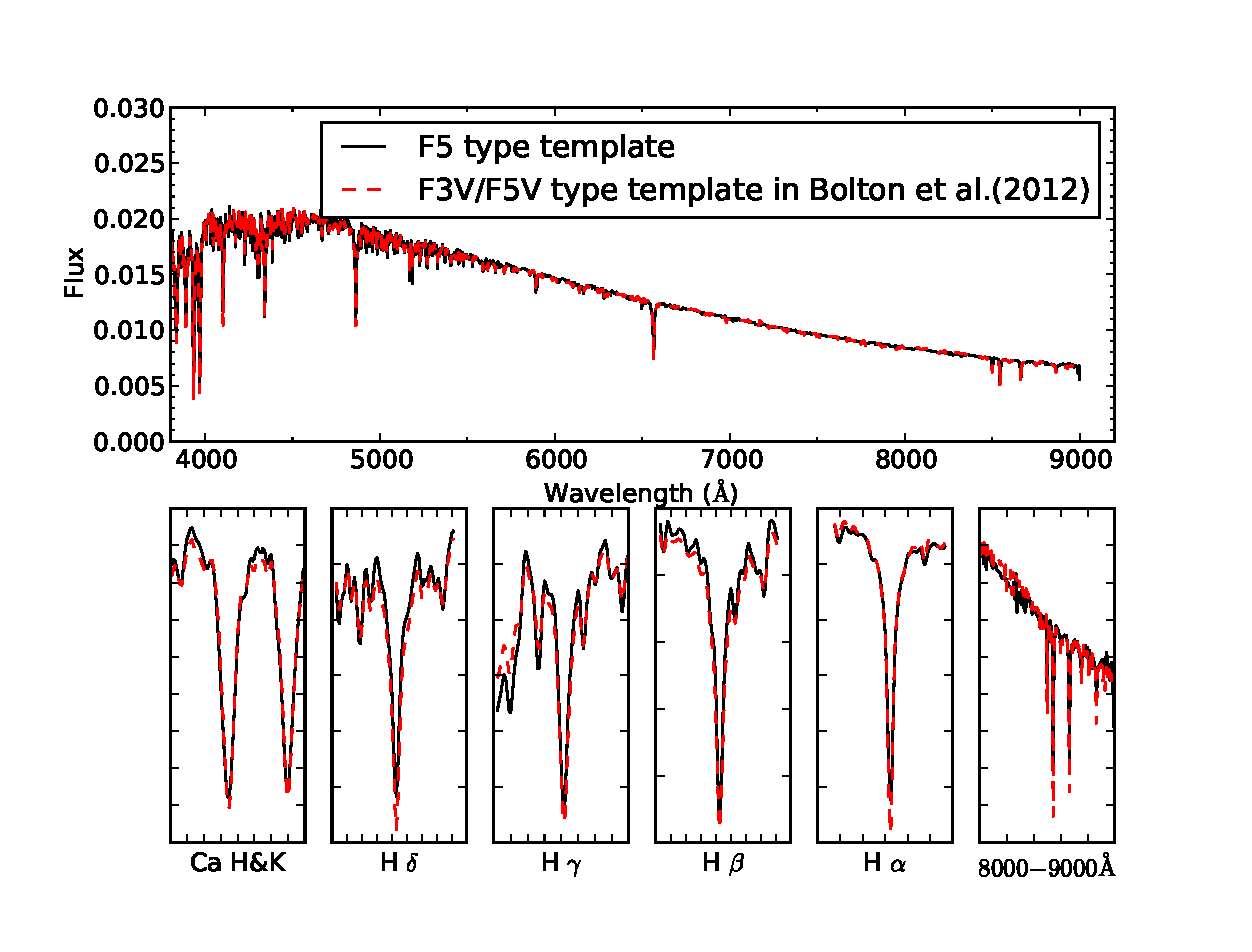
\includegraphics[width=14cm, angle=0,clip]{f91.eps}
   \caption{The comparison of the template spectrum \#69 with  F3V/F5V type spectrum  in  \citet{bolton2012spectral}.
The black line is the spectrum constructed in our work.
The red one is the closest spectrum in  \citet{bolton2012spectral}.
   }
   \label{Fig91}
\end{figure}

\begin{figure}
   \centering
   \includegraphics[width=14cm, angle=0,clip]{f72.eps}
   \caption{The first four eigen spectra (principal components) of group \#179.
   }
   \label{Fig72}
\end{figure}

 \begin{figure}
   \centering
   \includegraphics[width=14cm, angle=0,clip]{f82.eps}
   \caption{Three examples of reconstructed spectra in group \#179.
The black lines are the original spectra and the red lines are reconstructed spectra.
   }
   \label{Fig82}
\end{figure}
\begin{figure}
   \centering
   \includegraphics[width=14cm, angle=0,clip]{f92.eps}
   \caption{The comparison of the template spectrum \#34 with  A1IV type template in current library.
The black line is the spectrum constructed in our work.
The red one is the closest spectrum in current library.
   }
   \label{Fig92}
\end{figure}
\begin{figure}
   \centering
   \includegraphics[width=14cm, angle=0,clip]{f73.eps}
   \caption{The first four eigen spectra (principal components) of group \#204.
    Note that the strong lines in eigen spectra\#2 are emission lines not absorption lines.
   }
   \label{Fig73}
\end{figure}

 \begin{figure}
   \centering
   \includegraphics[width=14cm, angle=0,clip]{f83.eps}
   \caption{Three examples of reconstructed spectra in group \#204.
The black lines are the original spectra and the red lines are reconstructed spectra.
   }
   \label{Fig83}
\end{figure}




 \begin{figure}
   \centering
   \includegraphics[width=14cm, angle=0,clip]{f74.eps}
   \caption{The first four eigen spectra (principal components) of group \#222.
   }
   \label{Fig74}
\end{figure}

 \begin{figure}
   \centering
   \includegraphics[width=14cm, angle=0,clip]{f84.eps}
   \caption{Three examples of reconstructed spectra in group \#222.
   }
   \label{Fig84}
\end{figure}

 \begin{figure}
   \centering
   \includegraphics[width=14cm, angle=0,clip]{f94.eps}
   \caption{The comparison of the M2 type template spectrum \#159 with  M2 in   current LAMOST library and \citet{bochanski2007low}.
The black lines are the M2 type spectrum constructed in our work.
The red ones are the M2 type template in   current LAMOST library and \citet{bochanski2007low}.
   }
   \label{Fig94}
\end{figure}

%% edition.

%age when the default \tablewidth is used, as below.  The
%% individual table widths for each page will be written to the log file; a
%% maximum tablewidth
%
%\begin{deluxetable}{ccr}
%\tablecolumns{3}
%\tabletypesize{\scriptsize}
%%\setlength{\tabcolsep}{0.05in}
%\tablewidth{0pt}
%\tablecaption{The number distribution of different subclasses\label{tab1}}
%\tablehead{
%\colhead{Group ID}&
%\colhead{Subclass}&
%\colhead{Amount}
%}
%\startdata
%176	&A0	&94\\
%177	&A0I	&27\\
%178	&A0III	&407\\
%179	&A1IV	&653\\
%180	&A1V	&527\\
%181	&A2I	&10\\
%182	&A2IV	&1692\\
%183	&A2V	&5761\\
%184	&A3I	&37\\
%185	&A3IV	&2084\\
%186	&A3V	&2080\\
%187	&A4III	&926\\
%188	&A4V	&773\\
%189	&A5	&26\\
%190	&A5I	&213\\
%191	&A5V	&1253\\
%192	&A6IV	&1240\\
%193	&A6V	&322\\
%194	&A7III	&4033\\
%195	&A7V	&647\\
%196	&A9	&4\\
%197	&A9V	&2170\\
%198	&B	&15\\
%199	&B0	&1\\
%200	&B9	&443\\
%201	&Binary	&170\\
%202	&Carbon	&178\\
%203	&CarbonWD	&6\\
%204	&CV	&27\\
%205	&EM	&63\\
%206	&F0	&27808\\
%207	&F2	&44192\\
%208	&F5	&119328\\
%209	&F9	&292830\\
%210	&G0	&47697\\
%211	&G2	&92229\\
%212	&G5	&81202\\
%213	&G7	&3650\\
%214	&K0	&1998\\
%215	&K1	&85218\\
%216	&K3	&77164\\
%217	&K5	&73045\\
%218	&K7	&45839\\
%219	&K9	&4\\
%220	&M0	&19152\\
%221	&M1	&19953\\
%222	&M2	&17243\\
%223	&M3	&9749\\
%224	&M4	&3860\\
%225	&M5	&855\\
%226	&M6	&412\\
%227	&M7	&259\\
%228	&M8	&47\\
%229	&M9	&66\\
%230	&O	&79\\
%231	&OB	&16\\
%232	&WD	&535\\
%233	&WD Magnetic	&14\\
%
%\enddata
%
%\end{deluxetable}
%
%\clearpage


%% If the table is more than one page long, the width of the table can vary
%% from page to p for the table can be computed from these values.
%% The \tablewidth argument can then be reset and the file reprocessed, so
%% that the table is of uniform width throughout. Try getting the widths
%% from the log file and changing the \tablewidth parameter to see how
%% adjusting this value affects table formatting.

%% The \dataset{} macro has also been applied to a few of the objects to
%% show how many observations can be tagged in a table.



\clearpage

\begin{deluxetable}{cccccccc}
\tablecolumns{8}
\tabletypesize{\scriptsize}
%\setlength{\tabcolsep}{0.05in}
\tablewidth{0pt}
\tablecaption{The main inforamtion of the finally combined  template library \label{tab4}}
\tablehead{
\colhead{Spectra Type}&
\colhead{Subclass ID}&
\colhead{Subclass}&
\colhead{C1}&
\colhead{C2}&
\colhead{C3}&
\colhead{Template IDs}
}
\startdata
O	&1	&O	&1	&0	&1	&1\\
	&2	&OB	&1	&0	&1	&2\\
B	&3	&B2	&0	&4	&4	&3-6\\
	&4	&B3	&0	&2	&2	&7-8\\
	&5	&B5	&0	&2	&2	&9-10\\
	&6	&B6	&1	&1	&1	&11\\
	&7	&B8	&0	&15	&15	&12-26\\
	&8	&B9	&1	&2	&2	&27-28\\
A	&9	&A0	&1	&0	&1	&29\\
	&10	&A0I	&1	&1	&1	&30\\
	&11	&A0III	&1	&1	&1	&31\\
	&12	&A0V	&1	&0	&1	&32\\
	&13	&A1III	&1	&0	&1	&33\\
	&14	&A1IV	&1	&1	&1	&34\\
	&15	&A1V	&1	&1	&1	&35\\
	&16	&A2I	&1	&0	&1	&36\\
	&17	&A2IV	&1	&1	&1	&37\\
	&18	&A2V	&1	&1	&1	&38\\
	&19	&A3I	&1	&0	&1	&39\\
	&20	&A3IV	&1	&1	&1	&40\\
	&21	&A3V	&1	&1	&1	&41\\
	&22	&A4III	&1	&1	&1	&42\\
	&23	&A4V	&1	&1	&1	&43\\
	&24	&A5	&1	&0	&1	&44\\
	&25	&A5I	&1	&1	&1	&45\\
	&26	&A5V	&1	&1	&1	&46\\
	&27	&A6IV	&1	&1	&1	&47\\
	&28	&A6V	&1	&1	&1	&48\\
	&29	&A7III	&1	&1	&1	&49\\
	&30	&A7V	&1	&1	&1	&50\\
	&31	&A9	&1	&1	&1	&51\\
	&32	&A9V	&1	&1	&1	&52\\
F	&33	&F0	&1	&4	&4	&53-56\\
	&34	&F2	&1	&4	&4	&57-60\\
	&35	&F3/F5V	&0	&7	&7	&61-67\\
	&36	&F5	&1	&5	&5	&68-72\\
	&37	&F6V	&0	&1	&1	&73\\
	&38	&F8	&0	&1	&1	&74\\
	&39	&F9	&1	&2	&2	&75-76\\
G	&40	&G0	&1	&3	&3	&77-79\\
	&41	&G2	&1	&9	&9	&80-88\\
	&42	&G3V	&0	&1	&1	&89\\
	&43	&G4V	&0	&2	&2	&90-91\\
	&44	&G5	&1	&1	&1	&92\\
	&45	&G7V	&0	&4	&4	&93-96\\
	&46	&G8V	&0	&5	&5	&97-101\\
	&47	&G9	&0	&2	&2	&102-103\\
K	&48	&K0	&1	&1	&1	&104\\
	&49	&K1	&1	&6	&6	&105-110\\
	&50	&K3	&1	&9	&9	&111-119\\
	&51	&K5	&1	&9	&9	&120-128\\
	&52	&K7	&1	&11	&11	&129-139\\
M	&53	&M0	&1	&10	&10	&140-149\\
	&54	&M0V	&1	&0	&1	&150\\
	&55	&M1	&1	&7	&7	&151-157\\
	&56	&M2	&1	&2	&2	&158-159\\
	&57	&M2V	&1	&0	&1	&160\\
	&58	&M3	&1	&3	&3	&161-163\\
	&59	&M4	&1	&1	&1	&164\\
	&60	&M5	&1	&1	&1	&165\\
	&61	&M6	&1	&1	&1	&166\\
	&62	&M7	&1	&1	&1	&167\\
	&63	&M8	&1	&1	&1	&168\\
	&64	&M9	&1	&1	&1	&169\\
other	&65	&Carbon	&1	&1	&1	&170\\
	&66	&Carbon\_lines	&1	&1	&1	&171\\
	&67	&WD	&1	&1	&1	&172\\
	&68	&CarbonWD	&1	&0	&1	&173\\
	&69	&WDmagnetic	&1	&0	&1	&174\\
	&70	&Binary	&0	&1	&1	&175\\
	&71	&CV	&0	&1	&1	&176\\
sum	&	&	&57	&164	&176	&\\




\enddata
\tablecomments{C1 is the amount of templates with corresponding subclass in current library.
C2 is the amount of   templates with corresponding subclass in our constructed library.
C3 is the amount of   templates with corresponding subclass in the finally combined library.
}
\end{deluxetable}
\clearpage

\begin{deluxetable}{cccc}

\tablecolumns{4}
\tabletypesize{\scriptsize}
\setlength{\tabcolsep}{0.5in}
\tablewidth{400pt}
\tablecaption{Comparison with \citet{bolton2012spectral}\label{tab3}}
\tablehead{
\colhead{Spectra type}&
\colhead{A1}&
\colhead{A2}&
\colhead{A3}
}
\startdata
O	&3	&2	&2\\
B	&30	&6	&26\\
A	&19	&24	&24\\
F	&19	&7	&24\\
G	&15	&8	&27\\
K	&19	&5	&36\\
M	&12	&12	&30\\
Others	&6	&7	&7\\
\enddata
\tablecomments{A1 is the Amount of templates in  \citet{bolton2012spectral}.
A2 is amount of subclasses in final library and A3 is  the amount of templates in final library.
}
\end{deluxetable}
\clearpage
\begin{deluxetable}{cccccccc}
\tablecolumns{8}
\tabletypesize{\scriptsize}
%\setlength{\tabcolsep}{0.05in}
\tablewidth{0pt}
\tablecaption{The main information of template \#69, \#34, \#176, \#159\label{tab2}}
\tablehead{
\colhead{Template ID}&
\colhead{Group ID}&
\colhead{All spectra}&
\colhead{Used spectra}&
\colhead{Subclass}&
\colhead{Subclass1}&
\colhead{Subclass2}&
\colhead{Subclass3}
}
\startdata
69  &59  &18534    &3048  &F5V    &F3V/F5V  &F1V &F5   \\
34  &179 &653    &381  &A1IV    &A4V/A1V  &A2V&A1V    \\
176 &204 &27     &13  &CV    &-  &-&-    \\
159 &222 &17231     &325  &M2    &M1/M0  &M1.5V/M3V&M2/M1    \\
\enddata
\tablecomments{Subclass is the finally labeled MK class.
Subclass2 is the best fit MK class with  \citet{danks1994atlas}.
Subclass3 is the best fit MK class with  \citet{luo2012dr1}.}
\end{deluxetable}
\clearpage
%% Tables may also be prepared as separate files. See the accompanying
%% sample file table.tex for an example of an external table file.
%% To include an external file in your main document, use the \input
%% command. Uncomment the line below to include table.tex in this
%% sample file. (Note that you will need to comment out the \documentclass,
%% \begin{document}, and \end{document} commands from table.tex if you want
%% to include it in this document.)

%% \input{table}

%% The following command ends your manuscript. LaTeX will ignore any text
%% that appears after it.

\end{document}

%%
%% End of file `sample.tex'.
